\documentclass[11pt,a4paper]{article}

% --- Paquetes compatibles con pdfLaTeX (estándar de Overleaf) ---
\usepackage[utf8]{inputenc}
\usepackage[T1]{fontenc}
\usepackage{lmodern}
\usepackage[spanish,es-tabla]{babel}
\usepackage[margin=2.5cm]{geometry}
\usepackage{xcolor}
\usepackage{graphicx}
\usepackage{tabularx}
\usepackage{booktabs}
\usepackage{longtable}
\usepackage{array}
\usepackage{enumitem}
\usepackage{fancyhdr}
\usepackage{titlesec}
\usepackage[hidelinks]{hyperref}

\graphicspath{{figuras/}}

% --- Páginas de flotantes alineadas arriba (no centradas verticalmente) ---
\makeatletter
\setlength{\@fptop}{0pt}
\setlength{\@fpsep}{1.5\baselineskip}
\makeatother

% --- Colores corporativos ULPGC ---
\definecolor{ulpgcblue}{RGB}{0, 102, 161}
\definecolor{ulpgcorange}{RGB}{243, 146, 0}
\definecolor{lightgray}{RGB}{245, 247, 250}

% --- Formato de títulos ---
\titleformat{\section}
  {\normalfont\Large\bfseries\color{ulpgcblue}}{\thesection}{1em}{}
\titleformat{\subsection}
  {\normalfont\large\bfseries\color{ulpgcblue!85!black}}{\thesubsection}{1em}{}
\titleformat{\subsubsection}
  {\normalfont\normalsize\bfseries\color{black!80}}{\thesubsubsection}{1em}{}

% --- Encabezado y pie de página ---
\pagestyle{fancy}
\fancyhf{}
\setlength{\headheight}{14pt}
\fancyhead[L]{\footnotesize\textcolor{gray}{ULPGC -- EII | Programación de Aplicaciones Móviles Nativas}}
\fancyhead[R]{\footnotesize\textcolor{gray}{Trabajo Final PAMN}}
\fancyfoot[C]{\thepage}
\renewcommand{\headrulewidth}{0.4pt}

% --- Configuración de tablas ---
\renewcommand{\arraystretch}{1.35}
\newcolumntype{L}[1]{>{\raggedright\arraybackslash}p{#1}}
\newcolumntype{Y}{>{\raggedright\arraybackslash}X}

\begin{document}

% ==========================================
% PORTADA
% ==========================================
\begin{titlepage}
    \centering
    \vspace*{1.5cm}
    {\Large\textbf{UNIVERSIDAD DE LAS PALMAS DE GRAN CANARIA}\par}
    \vspace{0.3cm}
    {\large Escuela de Ingeniería Informática\par}
    \vspace{0.2cm}
    {\normalsize Grado en Ingeniería Informática\par}

    \vspace{2.5cm}
    {\color{ulpgcblue}\rule{\linewidth}{1.5pt}\par}
    \vspace{0.4cm}
    {\Huge\bfseries\textcolor{ulpgcblue}{Cartelera de Cine}\par}
    \vspace{0.3cm}
    {\Large Memoria del Trabajo Final -- PAMN\par}
    \vspace{0.2cm}
    {\color{ulpgcblue}\rule{\linewidth}{1.5pt}\par}

    \vspace{2cm}
    \begin{flushleft}
        \textbf{Asignatura:} Programación de Aplicaciones Móviles Nativas\\
        \textbf{Plataforma y lenguaje:} Android (Kotlin)\\[0.4cm]
        \textbf{Integrantes del equipo:}
        \begin{itemize}[leftmargin=1.5cm]
            \item Alejandro Celis Hernández Delgado
            \item Joel Morera Apaza
        \end{itemize}
        \vspace{0.4cm}
        \textbf{Repositorio de GitHub:} \url{https://github.com/PAMN-Grupo08-ULPGC-Cartelera-de-Cine/Cartelera-Cine}\\
    \end{flushleft}

    \vfill
    {\large Las Palmas de Gran Canaria, \today\par}
\end{titlepage}

\tableofcontents
\newpage

% ==========================================
% 1. INTRODUCCIÓN Y OBJETIVOS
% ==========================================
\section{Introducción y objetivos}
\textit{Describir la aplicación, la necesidad o experiencia que ofrece, el público objetivo y los objetivos. Delimitar el alcance y las funcionalidades principales.}

\subsection{Descripción general y motivación}
[Texto descriptivo de la aplicación...]

\subsection{Público objetivo}
[Definición de los perfiles de usuario a los que va dirigida la app...]

\subsection{Objetivos y alcance del proyecto}
\begin{itemize}
    \item \textbf{Objetivo general:} Diseñar e implementar una aplicación nativa en Android con Kotlin que permita...
    \item \textbf{Alcance funcional:} El recorrido principal cubre desde [inicio] hasta [fin]...
\end{itemize}

% ==========================================
% 2. ANÁLISIS DE REQUISITOS
% ==========================================
\section{Análisis de requisitos}
En este apartado se presentan los actores del sistema, los requisitos funcionales y no funcionales (identificados de forma única y con criterios de verificación concretos), las historias de usuario y los casos de uso principales que guían el desarrollo. Cada requisito se relaciona con los casos de prueba del apartado~\ref{sec:pruebas}.

\subsection{Identificación de actores}
\begin{table}[htbp]
\centering
\begin{tabularx}{\textwidth}{L{1.8cm} L{2.8cm} Y}
\toprule
\textbf{ID} & \textbf{Actor} & \textbf{Descripción y rol en la aplicación} \\
\midrule
\textbf{ACT-01} & Cliente & Persona que consulta la cartelera y compra entradas. Antes de iniciar sesión solo puede registrarse o autenticarse; una vez autenticado puede reservar asientos, pagar y consultar sus entradas. \\
\midrule
\textbf{ACT-02} & Empleado & Trabajador del cine. Se registra con un código de empleado y, una vez autenticado, valida las entradas escaneando su código QR en el acceso a la sala. \\
\midrule
\textbf{ACT-03} & Temporizador (sistema) & Tarea periódica del servidor que libera los asientos de las reservas no pagadas dentro del plazo establecido. \\
\bottomrule
\end{tabularx}
\caption{Actores identificados en el sistema.}
\label{tab:actores}
\end{table}

\subsection{Requisitos funcionales (RF)}
Cada requisito funcional tiene una prioridad (Alta, Media o Baja) y un criterio de verificación que se comprueba en el apartado de pruebas.

\begin{longtable}{L{1.3cm} L{2.6cm} L{4.6cm} L{1.3cm} L{4.0cm}}
\caption{Requisitos funcionales.}\label{tab:rf}\\
\toprule
\textbf{ID} & \textbf{Nombre} & \textbf{Descripción} & \textbf{Prior.} & \textbf{Criterio de verificación} \\
\midrule
\endfirsthead
\toprule
\textbf{ID} & \textbf{Nombre} & \textbf{Descripción} & \textbf{Prior.} & \textbf{Criterio de verificación} \\
\midrule
\endhead
\bottomrule
\endlastfoot

\textbf{RF-01} & Registro de usuario & El sistema debe permitir crear una cuenta con nombre, correo y contraseña. Si se introduce un código de empleado válido, la cuenta se crea con rol Empleado. & Alta & Con datos válidos (correo con formato correcto, contraseña de al menos 8 caracteres) se crea la cuenta y se inicia sesión. Si el correo ya existe o el código de empleado no es válido, se muestra un mensaje de error específico junto al campo afectado. \\
\midrule
\textbf{RF-02} & Inicio de sesión & El usuario registrado debe poder iniciar sesión con correo y contraseña. & Alta & Con credenciales correctas se navega a la cartelera (rol Cliente) o a la pantalla de escaneo (rol Empleado). Con credenciales incorrectas se muestra «Correo o contraseña incorrectos» sin revelar cuál de los dos falla. \\
\midrule
\textbf{RF-03} & Cierre de sesión & El usuario autenticado debe poder cerrar su sesión desde la pantalla de perfil. & Media & Se eliminan los datos de sesión del dispositivo, se redirige al login y el botón «Atrás» del sistema no permite volver a pantallas autenticadas. \\
\midrule
\textbf{RF-04} & Cartelera & La aplicación debe mostrar las películas con sesiones disponibles, obtenidas del servidor y almacenadas en caché local. & Alta & Se muestra un indicador de carga durante la consulta. Sin conexión se muestran los datos en caché con un aviso; sin caché ni conexión se muestra un estado de error con opción de reintentar. \\
\midrule
\textbf{RF-05} & Búsqueda y filtrado de películas & El usuario podrá filtrar la cartelera por título y por género. & Media & La lista se actualiza al escribir, sin distinguir mayúsculas ni tildes. Si ningún título coincide, se muestra «No hay películas que coincidan». \\
\midrule
\textbf{RF-06} & Detalle de película & Al seleccionar una película se mostrará su sinopsis, duración, género, clasificación por edad y sesiones disponibles. & Alta & Se navega con el identificador de la película y se muestran todos los campos indicados y las sesiones ordenadas por fecha y hora. \\
\midrule
\textbf{RF-07} & Selección y reserva de asientos & El cliente podrá elegir uno o varios asientos (máximo 8) en el mapa de la sala de una sesión. Al confirmar, los asientos quedan bloqueados temporalmente a su nombre. & Alta & Los asientos ocupados o bloqueados no son seleccionables. Al confirmar, los asientos quedan reservados durante 8 minutos. Si otro usuario ha reservado alguno de ellos antes, se informa «Algún asiento ya no está disponible» y se refresca el mapa. \\
\midrule
\textbf{RF-08} & Pago simulado & El cliente podrá confirmar el pago de una reserva vigente mediante un formulario de pago simulado. & Alta & Si la reserva no ha caducado, se generan las entradas y se muestra la confirmación. Si ha caducado, se informa y se vuelve a la selección de asientos. Un reintento por fallo de red no genera entradas duplicadas. \\
\midrule
\textbf{RF-09} & Mis entradas & El cliente podrá consultar sus entradas compradas con su código QR. & Alta & Las entradas y sus QR se muestran también sin conexión si se han consultado antes. \\
\midrule
\textbf{RF-10} & Validación de entradas & El empleado podrá escanear el código QR de una entrada con la cámara para validarla. & Alta & Una entrada válida se marca como usada y se muestra en verde. Una entrada ya usada, falsificada o de otra sesión se rechaza y se muestra en rojo con el motivo. \\
\midrule
\textbf{RF-11} & Liberación de reservas caducadas & El sistema liberará automáticamente los asientos de las reservas no pagadas en el plazo establecido. & Alta & Pasados 8 minutos sin pago, los asientos vuelven a estar disponibles para otros usuarios. \\
\end{longtable}

\subsection{Requisitos no funcionales (RNF)}
Los requisitos no funcionales recogen los criterios de calidad técnica, arquitectura, concurrencia, seguridad y usabilidad del proyecto.

\begin{longtable}{L{1.6cm} L{2.8cm} L{5.0cm} L{4.6cm}}
\caption{Requisitos no funcionales.}\label{tab:rnf}\\
\toprule
\textbf{ID} & \textbf{Categoría} & \textbf{Descripción} & \textbf{Métrica / verificación} \\
\midrule
\endfirsthead
\toprule
\textbf{ID} & \textbf{Categoría} & \textbf{Descripción} & \textbf{Métrica / verificación} \\
\midrule
\endhead
\bottomrule
\endlastfoot

\textbf{RNF-01} & Arquitectura & La aplicación separa responsabilidades entre la interfaz, la lógica de presentación, la lógica de negocio y el acceso a datos. & Los componentes de interfaz no acceden directamente a la red ni a la base de datos. \\
\midrule
\textbf{RNF-02} & Asincronía & Las operaciones de red y base de datos se ejecutan sin bloquear el hilo principal. & La interfaz sigue respondiendo durante las cargas; ausencia de errores ANR durante las pruebas. \\
\midrule
\textbf{RNF-03} & Consistencia en compras concurrentes & Un mismo asiento de una sesión nunca puede venderse dos veces, aunque varios usuarios lo reserven a la vez. & Test de integración que lanza 50 reservas simultáneas del mismo asiento: exactamente una tiene éxito y el resto se rechaza indicando que el asiento no está disponible. \\
\midrule
\textbf{RNF-04} & Escalabilidad & El sistema debe atender a muchos usuarios simultáneos sin perder la consistencia de los datos. & Prueba de carga con usuarios concurrentes sin errores ni ventas duplicadas. \\
\midrule
\textbf{RNF-05} & Seguridad & Las contraseñas no se almacenan en claro, las operaciones privadas requieren estar autenticado y los códigos QR no pueden falsificarse. & No hay contraseñas legibles en el almacenamiento; una operación privada sin autenticar se rechaza; un QR modificado se rechaza al validarlo. \\
\midrule
\textbf{RNF-06} & Funcionamiento sin conexión & La cartelera y las entradas compradas están disponibles sin conexión a partir de la última sincronización. & Con el modo avión activado se muestran la cartelera en caché y el QR de las entradas. \\
\midrule
\textbf{RNF-07} & Gestión de estados y errores & Todas las pantallas con datos asíncronos contemplan los estados de carga, éxito, vacío y error. & Ante pérdida de conexión la app no se cierra y muestra un mensaje con opción de reintentar. \\
\midrule
\textbf{RNF-08} & Rendimiento & La validación de una entrada debe resolverse con rapidez para no formar colas en el acceso. & Con conexión estable, el resultado de la validación se muestra en menos de 2 segundos desde la lectura del QR. \\
\midrule
\textbf{RNF-09} & Usabilidad y accesibilidad & Interfaz consistente y legible, con contraste adecuado, áreas táctiles de al menos 48\,dp, descripciones de contenido y soporte del tamaño de fuente del sistema. & Revisión con Accessibility Scanner y con el tamaño de fuente del sistema al máximo sin texto cortado. \\
\midrule
\textbf{RNF-10} & Seguridad del repositorio & Las claves, secretos y ficheros de configuración sensibles no se suben al control de versiones. & Revisión del historial de GitHub: el repositorio solo contiene ficheros de ejemplo sin credenciales reales. \\
\end{longtable}

\subsection{Historias de usuario (HU)}
Las historias de usuario sirven como base para los \textit{issues} y la planificación del tablero en GitHub. Cada historia indica los requisitos funcionales con los que se relaciona.

\begin{longtable}{L{2.8cm} L{5.8cm} L{6.1cm}}
\caption{Historias de usuario.}\label{tab:hu}\\
\toprule
\textbf{ID y nombre} & \textbf{Historia} & \textbf{Criterios de aceptación} \\
\midrule
\endfirsthead
\toprule
\textbf{ID y nombre} & \textbf{Historia} & \textbf{Criterios de aceptación} \\
\midrule
\endhead
\bottomrule
\endlastfoot

\textbf{HU-01}\newline Registro de cliente\newline{\small(RF-01)} & \textbf{Como} cliente nuevo, \textbf{quiero} registrarme con mi correo \textbf{para} poder comprar entradas y conservarlas en mi cuenta. & 1. El correo debe tener un formato válido.\newline 2. La contraseña debe tener al menos 8 caracteres.\newline 3. Si el correo ya está registrado, se muestra un error junto al campo.\newline 4. Tras registrarse, accede directamente a la cartelera. \\
\midrule
\textbf{HU-02}\newline Registro de empleado\newline{\small(RF-01)} & \textbf{Como} empleado del cine, \textbf{quiero} registrarme con el código de empleado que me facilita el cine \textbf{para} acceder a la validación de entradas. & 1. Con un código válido, la cuenta se crea con rol Empleado.\newline 2. Con un código no válido, se muestra un error y no se crea la cuenta.\newline 3. Sin código, la cuenta se crea como Cliente. \\
\midrule
\textbf{HU-03}\newline Inicio y cierre de sesión\newline{\small(RF-02, RF-03)} & \textbf{Como} usuario registrado, \textbf{quiero} iniciar y cerrar sesión \textbf{para} usar la app con mi cuenta y proteger mis datos en dispositivos compartidos. & 1. Un cliente entra a la cartelera y un empleado a la pantalla de escaneo.\newline 2. Con credenciales incorrectas se muestra «Correo o contraseña incorrectos».\newline 3. Al cerrar sesión no se puede volver atrás a pantallas privadas. \\
\midrule
\textbf{HU-04}\newline Consulta y búsqueda en cartelera\newline{\small(RF-04, RF-05)} & \textbf{Como} cliente, \textbf{quiero} ver la cartelera y buscar películas por título o género \textbf{para} decidir rápidamente qué ver. & 1. Se muestra un indicador mientras cargan las películas.\newline 2. Sin conexión se muestra la última cartelera guardada con un aviso.\newline 3. La búsqueda filtra al escribir, sin distinguir mayúsculas ni tildes.\newline 4. Si no hay coincidencias, se muestra un mensaje. \\
\midrule
\textbf{HU-05}\newline Detalle de película y sesiones\newline{\small(RF-06)} & \textbf{Como} cliente, \textbf{quiero} ver el detalle de una película y sus sesiones \textbf{para} elegir el día y la hora que me convienen. & 1. Se muestran sinopsis, duración, género y clasificación por edad.\newline 2. Las sesiones aparecen ordenadas por fecha y hora.\newline 3. Las sesiones completas aparecen marcadas y no se pueden seleccionar. \\
\midrule
\textbf{HU-06}\newline Selección y reserva de asientos\newline{\small(RF-07, RF-11)} & \textbf{Como} cliente, \textbf{quiero} elegir mis asientos en el mapa de la sala \textbf{para} sentarme donde prefiero con la seguridad de que nadie más los comprará mientras pago. & 1. Los asientos ocupados no se pueden seleccionar.\newline 2. Se pueden seleccionar hasta 8 asientos.\newline 3. \textbf{Dado} que otro usuario reserva un asiento antes que yo, \textbf{cuando} confirmo, \textbf{entonces} se me avisa y el mapa se actualiza.\newline 4. Se muestra el tiempo restante de la reserva (8 minutos). \\
\midrule
\textbf{HU-07}\newline Pago de la reserva\newline{\small(RF-08)} & \textbf{Como} cliente, \textbf{quiero} pagar mi reserva \textbf{para} obtener mis entradas. & 1. Con la reserva vigente, el pago genera una entrada por asiento.\newline 2. \textbf{Dado} que la reserva ha caducado, \textbf{cuando} intento pagar, \textbf{entonces} se me informa y vuelvo al mapa de asientos.\newline 3. Si falla la red y reintento, no se duplican las entradas. \\
\midrule
\textbf{HU-08}\newline Consulta de mis entradas\newline{\small(RF-09)} & \textbf{Como} cliente, \textbf{quiero} consultar mis entradas con su código QR \textbf{para} enseñarlas en la entrada del cine aunque no tenga cobertura. & 1. Se listan las entradas con película, sala, fecha, hora y asiento.\newline 2. El QR se muestra también sin conexión.\newline 3. Las entradas ya usadas aparecen marcadas como tales. \\
\midrule
\textbf{HU-09}\newline Validación de entradas por QR\newline{\small(RF-10)} & \textbf{Como} empleado, \textbf{quiero} escanear el QR de una entrada \textbf{para} permitir el acceso solo a quien tenga una entrada válida. & 1. Una entrada válida se muestra en verde y queda marcada como usada.\newline 2. Una entrada ya usada se muestra en rojo con la hora de su primer uso.\newline 3. Un QR falso o de otra sesión se rechaza y se indica el motivo.\newline 4. Si se niega el permiso de cámara, se explica cómo concederlo. \\
\end{longtable}

\subsection{Diagrama de casos de uso}
La figura~\ref{fig:casos-uso} resume los casos de uso de cada actor. Las relaciones \textit{«include»} indican pasos que siempre forman parte del caso base: seleccionar asientos siempre los bloquea temporalmente, pagar siempre genera el QR de la entrada y escanear un QR siempre implica validarlo en el servidor.

\begin{figure}[htbp]
\centering
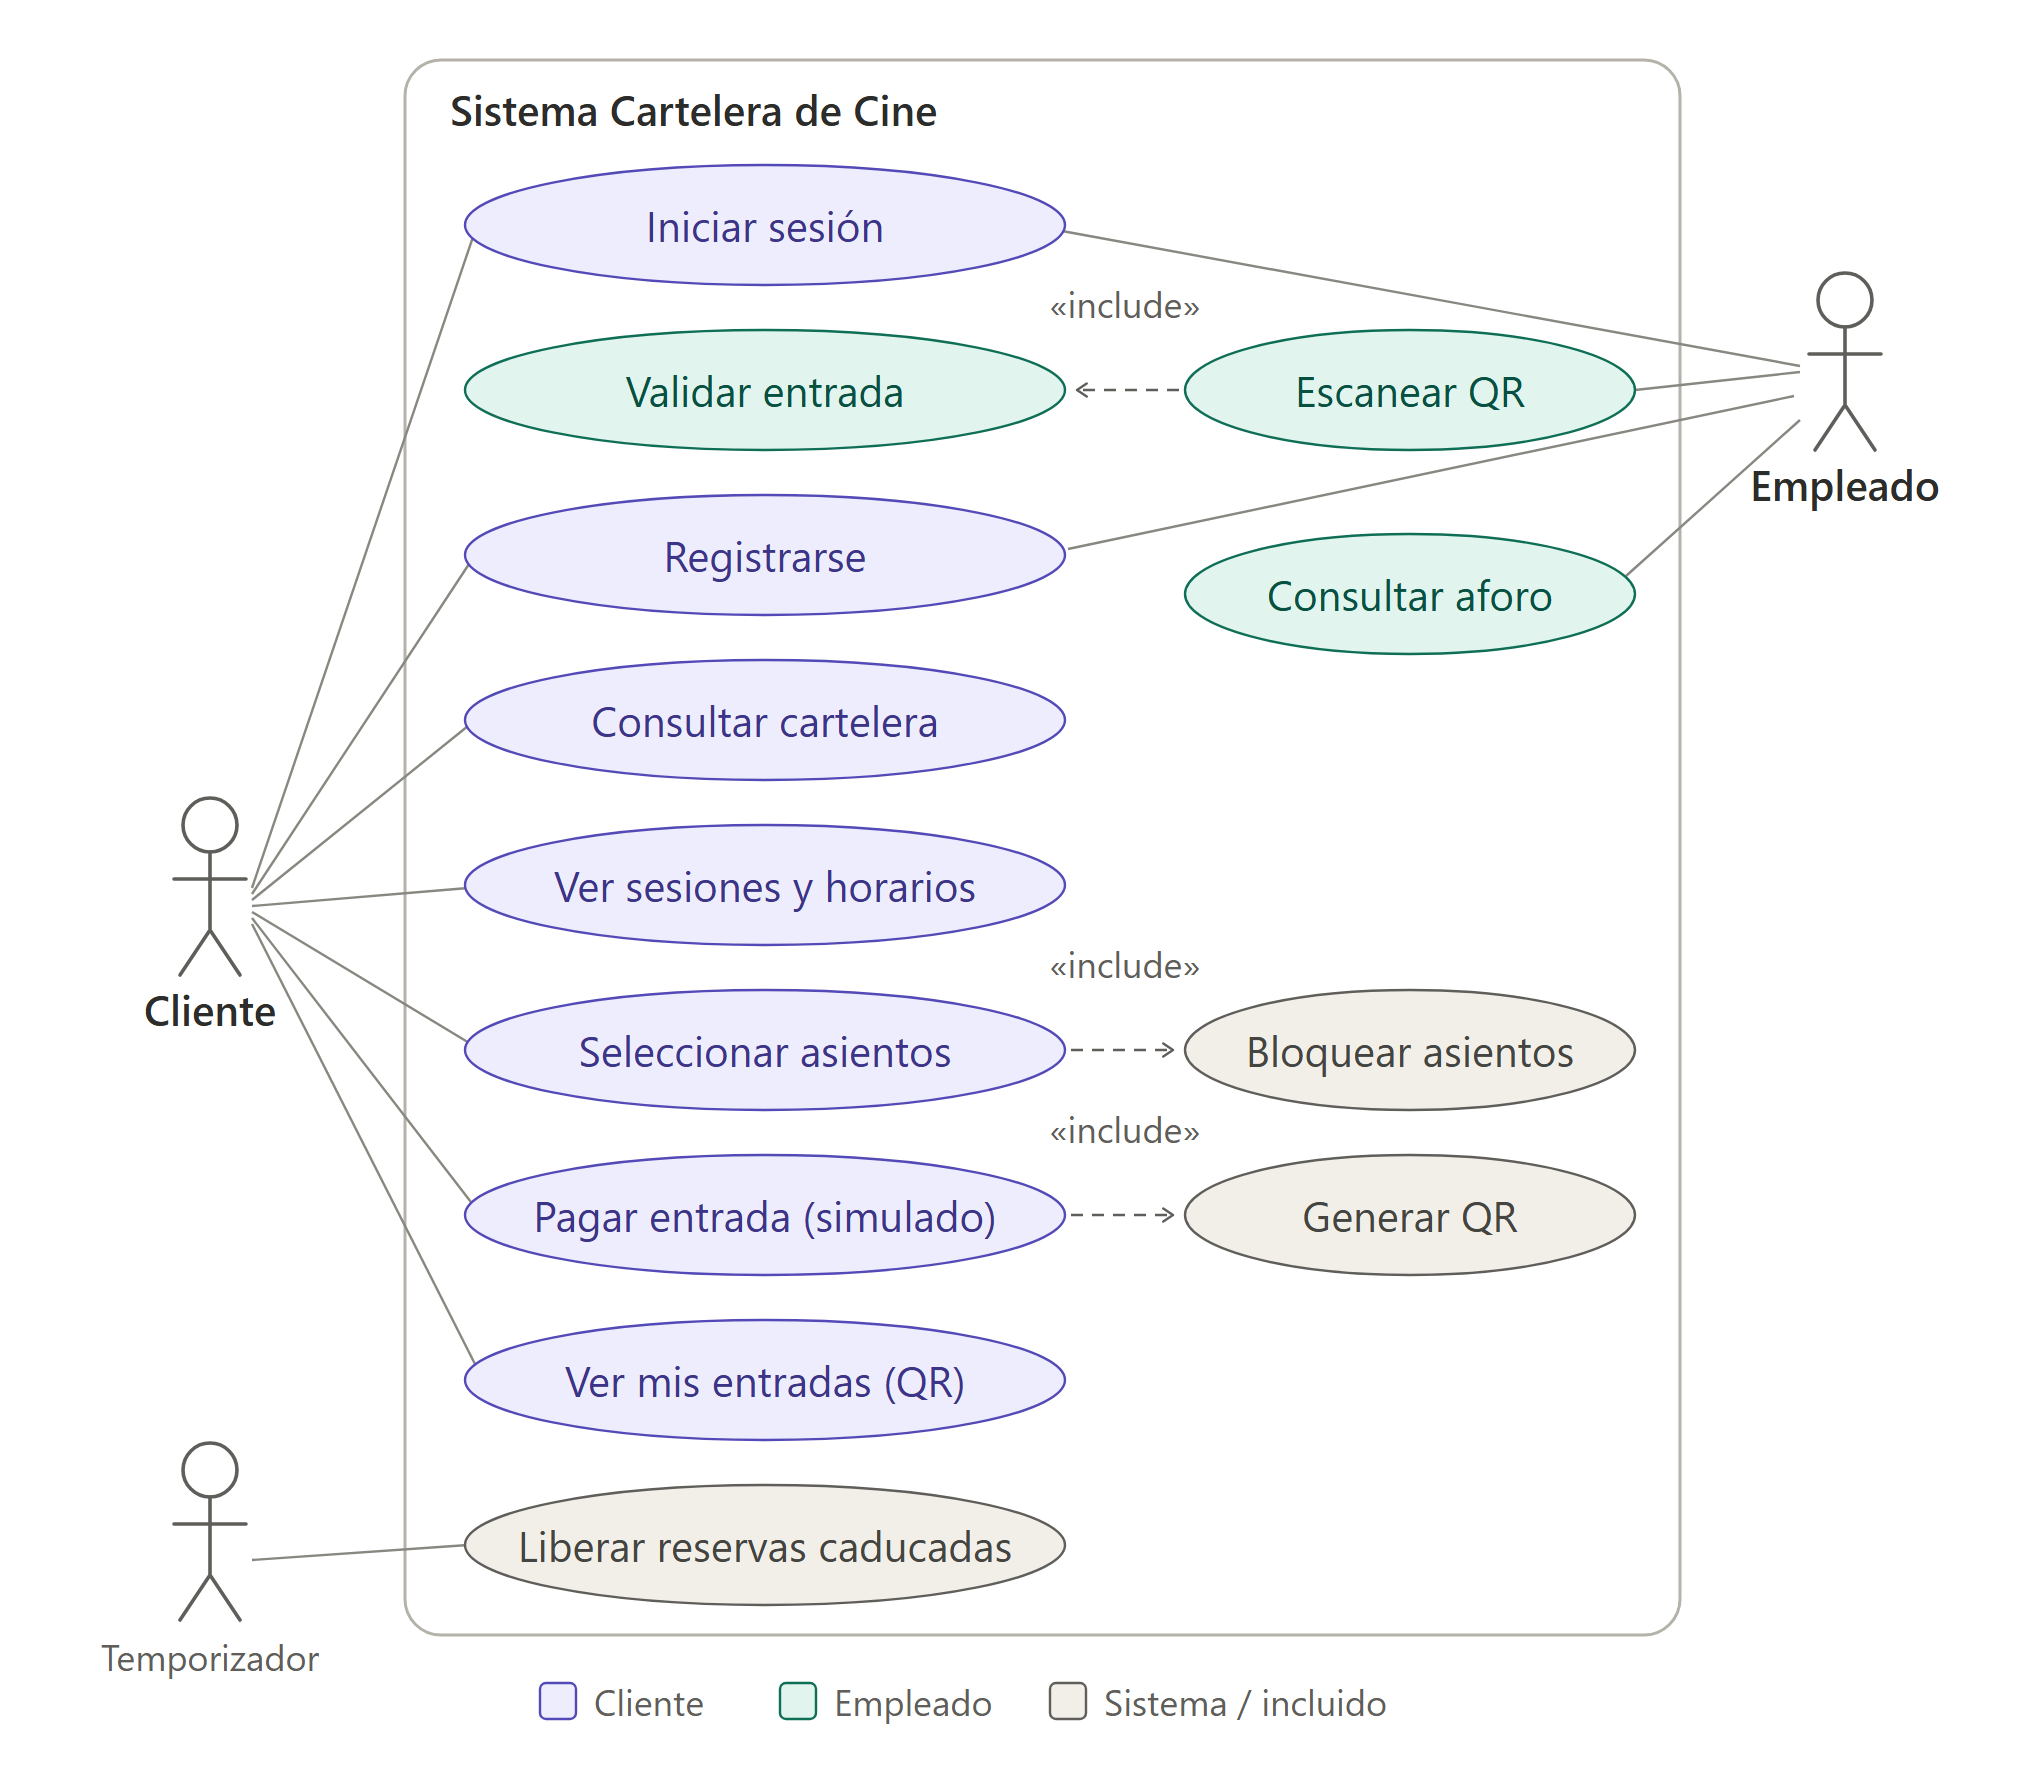
\includegraphics[width=0.9\textwidth]{casos-de-uso.png}
\caption{Diagrama de casos de uso (provisional).}
\label{fig:casos-uso}
\end{figure}

\subsection{Especificación de casos de uso (CU)}
A continuación se detallan los dos casos de uso críticos de la aplicación, con su flujo principal y el tratamiento de las situaciones de error.

\begin{table}[htbp]
\centering
\begin{tabularx}{\textwidth}{L{3.6cm} Y}
\toprule
\multicolumn{2}{l}{\textbf{CU-01: Comprar entradas para una sesión}} \\
\midrule
\textbf{Requisitos asociados} & RF-07, RF-08, RF-11, RNF-03 \\
\textbf{Actor principal} & ACT-01 (Cliente) \\
\textbf{Precondiciones} & El cliente ha iniciado sesión y se encuentra en el detalle de una película con sesiones disponibles. \\
\textbf{Flujo principal} &
1. El cliente selecciona una sesión.\newline
2. La aplicación muestra el mapa de la sala con los asientos libres, ocupados y bloqueados.\newline
3. El cliente selecciona uno o varios asientos (máximo 8) y pulsa «Continuar».\newline
4. El servidor bloquea los asientos a nombre del cliente durante 8 minutos y la aplicación muestra el resumen con el tiempo restante.\newline
5. El cliente introduce los datos del pago simulado y pulsa «Pagar».\newline
6. El servidor confirma la reserva y genera una entrada con código QR por cada asiento.\newline
7. La aplicación guarda las entradas en el dispositivo y muestra la confirmación. \\
\textbf{Flujos alternativos} &
\textbf{1a. Sesión completa:} la sesión aparece marcada y no se puede seleccionar.\newline
\textbf{4a. Asiento ocupado por otro usuario:} el servidor rechaza la reserva completa (conflicto), la aplicación muestra «Algún asiento ya no está disponible» y refresca el mapa sin perder el resto de la selección.\newline
\textbf{5a. Reserva caducada:} si han pasado los 8 minutos, los asientos se liberan (RF-11); al pagar se informa al cliente y se vuelve al mapa de asientos.\newline
\textbf{6a. Fallo de red durante el pago:} se muestra un error con opción de reintentar; un reintento del mismo pago no duplica las entradas. \\
\textbf{Postcondiciones} & Los asientos quedan vendidos y no pueden reservarse de nuevo; el cliente dispone de sus entradas en «Mis entradas», también sin conexión. \\
\bottomrule
\end{tabularx}
\caption{Especificación del caso de uso CU-01.}
\label{tab:cu01}
\end{table}

\begin{table}[htbp]
\centering
\begin{tabularx}{\textwidth}{L{3.6cm} Y}
\toprule
\multicolumn{2}{l}{\textbf{CU-02: Validar una entrada en el acceso}} \\
\midrule
\textbf{Requisitos asociados} & RF-10, RNF-05, RNF-08 \\
\textbf{Actor principal} & ACT-02 (Empleado) \\
\textbf{Precondiciones} & El empleado ha iniciado sesión y la aplicación tiene permiso para usar la cámara. \\
\textbf{Flujo principal} &
1. El empleado abre la pantalla de escaneo.\newline
2. El empleado enfoca el código QR que muestra el cliente.\newline
3. La aplicación lee el código y lo envía al servidor.\newline
4. El servidor comprueba la firma del código y marca la entrada como usada.\newline
5. La aplicación muestra el resultado en verde con la película, la sala y el asiento, y queda lista para el siguiente escaneo. \\
\textbf{Flujos alternativos} &
\textbf{1a. Permiso de cámara denegado:} se explica para qué se necesita la cámara y cómo concederlo desde los ajustes.\newline
\textbf{4a. Entrada ya usada:} se muestra en rojo «Entrada ya utilizada» con la hora de su primer uso.\newline
\textbf{4b. QR falsificado o de otra sesión:} se muestra en rojo el motivo del rechazo.\newline
\textbf{4c. Sin conexión:} no se puede validar; se muestra un aviso para reintentar cuando vuelva la conexión. \\
\textbf{Postcondiciones} & La entrada queda marcada como usada y no puede volver a validarse, aunque dos empleados la escaneen a la vez. \\
\bottomrule
\end{tabularx}
\caption{Especificación del caso de uso CU-02.}
\label{tab:cu02}
\end{table}

% ==========================================
% RESTO DE APARTADOS DE LA RÚBRICA (ESQUELETO)
% ==========================================
\section{Diseño de la interfaz y experiencia de usuario}
\textit{Mostrar las pantallas, su navegación y los prototipos iniciales. Justificar las decisiones de interacción y explicar los cambios respecto al diseño inicial. Considerar legibilidad, accesibilidad básica y adaptación a los dispositivos previstos.}

\subsection{Mapa de navegación}
\subsection{Prototipos iniciales y evolución del diseño}
\subsection{Accesibilidad, legibilidad y adaptación a pantallas}

\section{Arquitectura de la aplicación}
\textit{Identificar y justificar la arquitectura adoptada. Incluir un diagrama de componentes o capas, sus responsabilidades y su comunicación, relacionándolo con la implementación real.}

\subsection{Justificación del patrón arquitectónico (MVVM / Clean Architecture)}
\subsection{Diagrama de capas y flujo de datos}

\section{Gestión y persistencia de datos}
\textit{Explicar los datos y su modelo, relaciones y mecanismos de almacenamiento. Si existe base de datos, documentar su diseño. Si no es necesaria, justificarlo y describir la gestión del estado y de otros datos relevantes.}

\subsection{Modelo de datos y entidades}
\subsection{Estrategia de persistencia (local / remota)}

\section{Desarrollo e implementación}
\textit{Explicar la estructura de carpetas, ficheros y componentes principales, la gestión del estado, los patrones y las librerías. Describir la programación asíncrona utilizada (corrutinas en Kotlin). Documentar servicios, APIs o funciones del dispositivo y las decisiones técnicas relevantes.}

\subsection{Estructura de paquetes del proyecto}
\subsection{Gestión del estado reactivo y programación asíncrona (corrutinas)}
\subsection{Servicios externos, librerías y recursos del dispositivo}

\section{Pruebas y validación}\label{sec:pruebas}
\textit{Registrar casos de prueba con condiciones, acciones, resultado esperado y resultado obtenido. Identificar dispositivos o emuladores y versiones probadas, errores detectados y correcciones. Aportar evidencias de las funcionalidades principales y de errores relevantes; describir tests automatizados si los hay.}

\begin{table}[htbp]
\centering
\begin{tabularx}{\textwidth}{L{1.3cm} L{2.0cm} Y Y L{1.7cm}}
\toprule
\textbf{ID} & \textbf{Requisito} & \textbf{Condiciones y acción} & \textbf{Resultado esperado / obtenido} & \textbf{Estado} \\
\midrule
\textbf{CP-01} & RF-02 & Introducir un correo sin formato válido y pulsar «Iniciar sesión». & Se muestra un error de validación bajo el campo de correo. & Pendiente \\
\midrule
\textbf{CP-02} & RF-07, RNF-03 & Dos dispositivos seleccionan el mismo asiento de la misma sesión y confirman a la vez. & Solo uno obtiene la reserva; el otro ve «Algún asiento ya no está disponible» y el mapa actualizado. & Pendiente \\
\midrule
\textbf{CP-03} & RF-04, RNF-06 & Activar el modo avión y abrir la cartelera después de haberla consultado con conexión. & Se muestra la cartelera en caché con un aviso de falta de conexión, sin cierres inesperados. & Pendiente \\
\bottomrule
\end{tabularx}
\caption{Registro de pruebas funcionales y de error.}
\label{tab:pruebas}
\end{table}

\section{Proceso de desarrollo y gestión del proyecto}
\textit{Explicar etapas, organización del equipo, distribución de tareas y cambios de planificación. Incluir enlaces a issues, hitos, ramas y pull requests representativos y una síntesis de las aportaciones individuales.}

\subsection{Organización del equipo y reparto de tareas}
\subsection{Flujo de trabajo en GitHub (ramas, issues, hitos y pull requests)}

\section{Uso de herramientas de IA generativa}
\textit{Declarar si se ha utilizado IA. En caso afirmativo, identificar herramientas, finalidad, partes del proyecto afectadas y ejemplos representativos de instrucciones y resultados. Explicar cómo se revisaron, adaptaron y comprobaron las aportaciones.}

\section{Conclusiones y trabajo futuro}
\textit{Valorar el cumplimiento de los objetivos con referencia a los resultados. Explicar dificultades, aprendizajes, limitaciones y mejoras pendientes, diferenciándolas de las funcionalidades entregadas.}

\section*{Fuentes consultadas y referencias}
\addcontentsline{toc}{section}{Fuentes consultadas y referencias}
\begin{itemize}
    \item Documentación oficial de Android Developers: \url{https://developer.android.com}
    \item Guía de arquitectura de aplicaciones Android: \url{https://developer.android.com/topic/architecture}
\end{itemize}

\end{document}
